\documentclass[aspectratio=169]{beamer}

\usetheme{Madrid}
\usecolortheme{default}
\setbeamertemplate{navigation symbols}{}

\usepackage{amsmath}
\usepackage{amssymb}
\usepackage{graphicx}
\usepackage{booktabs}
\usepackage{tikz}
\usetikzlibrary{positioning, arrows.meta, shapes.geometric, fit, backgrounds, calc}
\usepackage{hyperref}
\graphicspath{{./}{figs/}}

\definecolor{successgreen}{RGB}{34,139,34}
\definecolor{failred}{RGB}{178,34,34}
\definecolor{simblue}{RGB}{70,130,180}

\newenvironment{tightitemize}{
  \begin{itemize}\setlength{\itemsep}{3pt}\setlength{\parskip}{0pt}}{\end{itemize}}

% tighter blocks: trim the gap after the title and between blocks (does not clip content)
\addtobeamertemplate{block begin}{}{\vspace{-3pt}}
\addtobeamertemplate{block end}{}{\vspace{-3pt}}

\title[Crane Control \& Calibration]{Crane Control Update and Sensor Calibration}
\subtitle{Policy$\to$PLC Interface, Tracking Accuracy, and Camera/Rack Calibration}
\author{George Sideris}
\institute{AML, McGill University \;|\; FPInnovations}
\date{June 2026}

\begin{document}

% ==================================================================
\begin{frame}
  \titlepage
\end{frame}

% ==================================================================
\begin{frame}{Outline}
\begin{enumerate}\setlength{\itemsep}{5pt}
  \item New control setup: policy $\to$ RelativeJointMover $\to$ PLC
  \item Position-error characterization over the rack (5 targets)
  \item Calibration: what we optimize (model-to-cloud ICP)
  \item Adapting William's code for both cameras
  \item Rack calibration: calibrated cameras + ArUco markers
  \item Updating the sim assets / poses to match real
  \item Next steps: train BC in sim, attempt zero-shot transfer
\end{enumerate}
\end{frame}

% ==================================================================
\begin{frame}{New Control Setup: Policy $\to$ RelativeJointMover $\to$ PLC}
\vspace{-3mm}
\begin{center}
\resizebox{0.64\textwidth}{!}{%
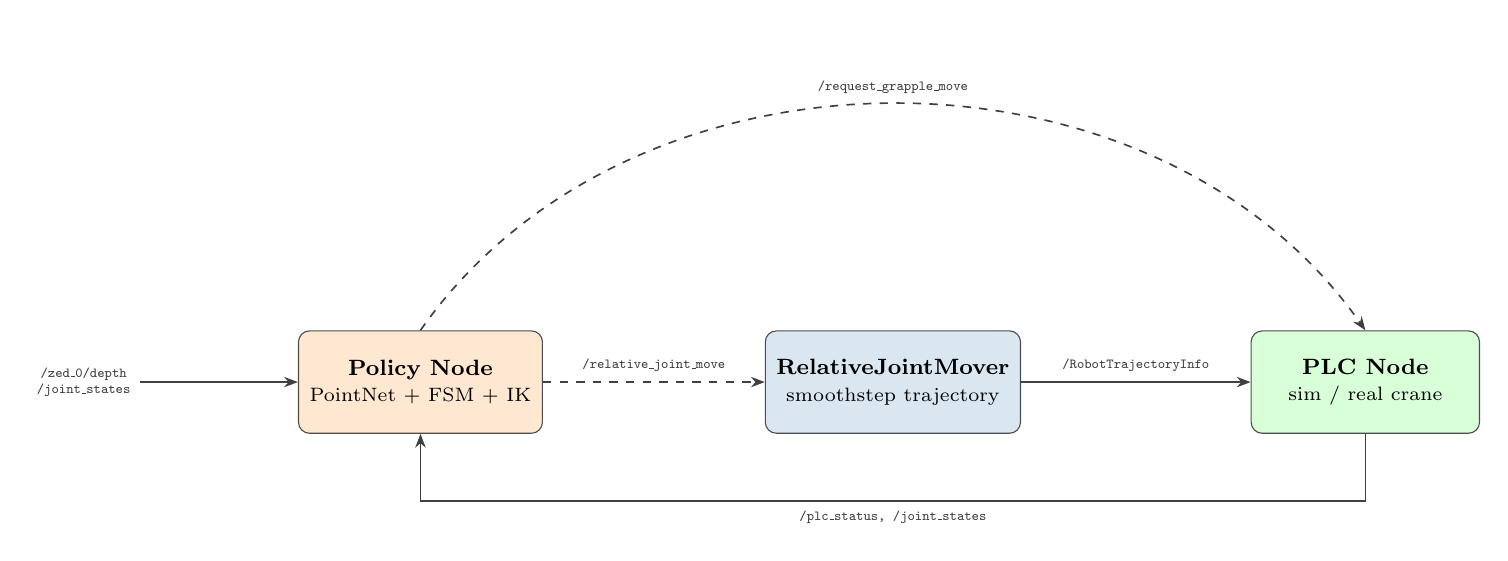
\begin{tikzpicture}[
  nd/.style={rectangle, rounded corners=4pt, draw=black!70,
    minimum width=2.9cm, minimum height=1.3cm, align=center,
    font=\footnotesize, inner sep=4pt},
  polnd/.style={nd, fill=orange!18},
  movnd/.style={nd, fill=simblue!20},
  ctrlnd/.style={nd, fill=green!15},
  tp/.style={font=\tiny\ttfamily, text=black!75, align=center},
  arr/.style={-{Stealth[length=5pt]}, semithick, black!75},
  sarr/.style={-{Stealth[length=5pt]}, semithick, black!75, dashed},
]
  \node[polnd] (pol) at (0,0) {\textbf{Policy Node}\\{\scriptsize PointNet + FSM + IK}};
  \node[movnd] (mov) at (6.0,0) {\textbf{RelativeJointMover}\\{\scriptsize smoothstep trajectory}};
  \node[ctrlnd] (plc) at (12.0,0) {\textbf{PLC Node}\\{\scriptsize sim / real crane}};

  % forward path
  \draw[sarr] (pol.east) -- node[above,tp]{/relative\_joint\_move} (mov.west);
  \draw[arr]  (mov.east) -- node[above,tp]{/RobotTrajectoryInfo} (plc.west);

  % gripper service (bypasses the mover), arc over the top
  \draw[sarr] (pol.north) to[out=55,in=125] node[above,tp]{/request\_grapple\_move} (plc.north);

  % sensor input
  \draw[arr] ([xshift=-2cm]pol.west) node[left,tp]{/zed\_0/depth\\/joint\_states} -- (pol.west);

  % feedback rail (bottom)
  \draw[arr] (plc.south) -- ([yshift=-0.85cm]plc.south)
    -- node[below,tp]{/plc\_status,\ /joint\_states} ([yshift=-0.85cm]pol.south) -- (pol.south);
\end{tikzpicture}%
}
\end{center}
\begin{columns}[t,totalwidth=\textwidth]
  \begin{column}{0.46\textwidth}
    \begin{block}{Policy Node (planning)}
      \scriptsize
      \begin{tightitemize}
        \item Depth $\to$ 1024-pt base-frame cloud $\to$ policy $\to$ $(x,y,z,\psi)$
        \item FSM per phase: IK $\to$ joint \emph{deltas} $\to$ \texttt{/relative\_joint\_move}; gripper $\to$ \texttt{/request\_grapple\_move}
        \item Advances on \texttt{/plc\_status} (HOLD/EXECUTE/END)
      \end{tightitemize}
    \end{block}
  \end{column}
  \begin{column}{0.46\textwidth}
    \begin{block}{RelativeJointMover (service)}
      \scriptsize
      \begin{tightitemize}
        \item Relative deltas + velocity + min duration; target $=$ current $+$ delta
        \item \textbf{7th-order smoothstep} (zero end velocity \& acceleration) at 50\,Hz --- hydraulic-friendly
        \item Publishes \texttt{RobotTrajectoryInfo}; same interface for sim \& real
      \end{tightitemize}
    \end{block}
  \end{column}
\end{columns}
\end{frame}

% ==================================================================
\begin{frame}{Position-Error Characterization (over the Rack)}
\vspace{-1mm}
\begin{columns}[c,totalwidth=\textwidth]
  \begin{column}{0.56\textwidth}
    \centering\footnotesize
    \begin{tabular}{ccc}
      \toprule
      \textbf{Target $(x,y,z)$} & \textbf{$\psi$} & \textbf{Task err (m)} \\
      \midrule
      $(-4.0,\,2.0,\,1.5)$ & $0.00$ & 0.014 \\
      $(-4.0,\,2.0,\,2.5)$ & $0.78$ & 0.018 \\
      $(-3.5,\,1.5,\,2.0)$ & $-0.78$ & 0.019 \\
      $(-3.5,\,2.5,\,2.0)$ & $1.57$ & 0.012 \\
      $(-4.5,\,2.0,\,2.0)$ & $-1.57$ & 0.010 \\
      \midrule
      \multicolumn{2}{r}{\textbf{mean / max}} & \textbf{0.015 / 0.019} \\
      \bottomrule
    \end{tabular}

    \vspace{2mm}
    {\scriptsize Each target: IK $\to$ \texttt{/relative\_joint\_move}; error from FK of the achieved joints vs.\ commanded EE.}
  \end{column}
  \begin{column}{0.42\textwidth}
    \begin{block}{Result}
      \footnotesize
      Over the rack workspace the crane tracks to \textbf{$\sim$1.5\,cm} (max 1.9\,cm); per-joint error $<0.005$\,rad, yaw error $<1.7^\circ$.
    \end{block}
    \vspace{-1mm}
    \begin{exampleblock}{Consistent Across the Rack}
      \footnotesize
      Accuracy holds across the swept height ($z = 1.5$--$2.5$\,m) and the full yaw range ($\psi = \pm\pi/2$), well within the grasp tolerance.
    \end{exampleblock}
  \end{column}
\end{columns}
\end{frame}

% ==================================================================
\begin{frame}{Calibrating the Basemast Camera}
\begin{columns}[c,totalwidth=\textwidth]
  \begin{column}{0.50\textwidth}
    \begin{block}{The Mount Is Adjustable}
      \small
      The policy consumes a point cloud in the crane \textbf{base frame}, so the real cloud must land in the same frame as the sim cloud it trained on. The basemast camera sits on a \textbf{repositionable magnet bracket} (and can shift on it), so its pose on the mast is not fixed --- it is \textbf{re-calibrated} directly to the mast whenever the mount moves.
    \end{block}
    \begin{block}{Sensors}
      \scriptsize
      \begin{tightitemize}
        \item \textbf{zed\_0} basemast (on the mast bracket, slews)
        \item \textbf{zed\_1} stick (on the stick)
        \item \textbf{lidar\_0} Ouster (same bracket; not used by the policy)
      \end{tightitemize}
    \end{block}
  \end{column}
  \begin{column}{0.46\textwidth}
    \begin{exampleblock}{Use the Grapple}
      \footnotesize
      The \textbf{grapple} \emph{does} move through the full workspace and is seen densely by both cameras --- use it as the calibration object.
    \end{exampleblock}
  \end{column}
\end{columns}
\end{frame}

% ==================================================================
\begin{frame}{Grapple-Based Mount Calibration (Model-to-Cloud ICP)}
\vspace{-1mm}
\begin{center}
\resizebox{0.92\textwidth}{!}{%
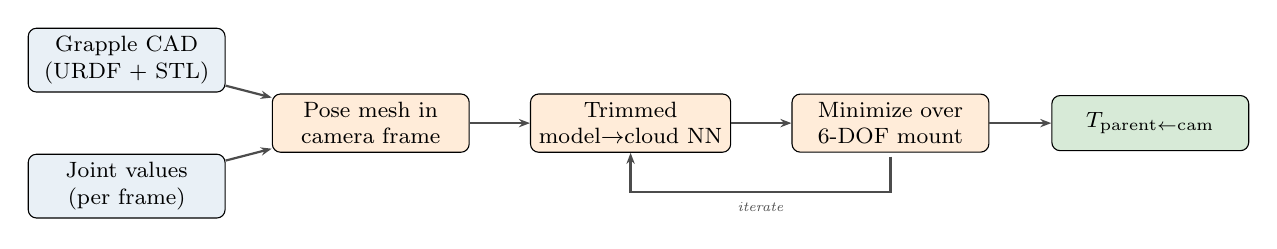
\begin{tikzpicture}[
  box/.style={draw, rounded corners=3pt, align=center, minimum width=2.5cm, minimum height=0.7cm, font=\footnotesize, inner sep=3pt},
  inb/.style={box, fill=simblue!12},
  opb/.style={box, fill=orange!15},
  outb/.style={box, fill=successgreen!18},
  arr/.style={-{Stealth[length=4pt]}, thick, black!70},
]
  \node[inb] (cad) at (0,0.8) {Grapple CAD\\(URDF + STL)};
  \node[inb] (jv) at (0,-0.8) {Joint values\\(per frame)};
  \node[opb] (pose) at (3.1,0) {Pose mesh in\\camera frame};
  \node[opb] (icp) at (6.4,0) {Trimmed\\model$\to$cloud NN};
  \node[opb] (opt) at (9.7,0) {Minimize over\\6-DOF mount};
  \node[outb] (out) at (13.0,0) {$T_{\text{parent}\leftarrow\text{cam}}$};
  \draw[arr] (cad) -- (pose); \draw[arr] (jv) -- (pose);
  \draw[arr] (pose) -- (icp); \draw[arr] (icp) -- (opt); \draw[arr] (opt) -- (out);
  \draw[arr] (opt.south) ++(0,-0.05) -- ++(0,-0.45) -| node[pos=0.25,below,font=\tiny\itshape]{iterate} (icp.south);
\end{tikzpicture}%
}
\end{center}
\vspace{-1mm}
\begin{columns}[t,totalwidth=\textwidth]
  \begin{column}{0.55\textwidth}
    \begin{block}{The Cost}
      \footnotesize
      Pose the grapple mesh by FK, project into the camera, and minimize the \textbf{trimmed model-to-cloud} nearest-neighbour squared distance over the 6-DOF mount $(x,y,z,\text{roll},\text{pitch},\text{yaw})$.
      \vspace{1mm}
      {\scriptsize Model$\to$cloud (not cloud$\to$model): the cropped cloud has non-grapple structure that the reverse direction diverges on.}
    \end{block}
  \end{column}
  \begin{column}{0.43\textwidth}
    \begin{block}{Accuracy Floor}
      \footnotesize
      RMS $\sim$47\,mm (zed\_1) / 64\,mm (zed\_0); higher for zed\_0's longer chain (sag, encoder error).
    \end{block}
    \begin{block}{Calibrated Mounts (full 6-DOF)}
      \scriptsize
      $T_{\text{mast}\leftarrow\text{zed\_0}}$: xyz $(-0.168,-0.014,0.897)$, rpy $(-106,-0.2,-1.9)^\circ$\\
      $T_{\text{stick}\leftarrow\text{zed\_1}}$: xyz $(-0.133,0.318,-0.009)$, rpy $(-90,0.6,-2.3)^\circ$\\
      {\tiny large roll $=$ camera optical-frame convention ($+Z$ forward)}
    \end{block}
  \end{column}
\end{columns}
\end{frame}

% ==================================================================
\begin{frame}{Adapting William's Code for Both Cameras}
\begin{columns}[c,totalwidth=\textwidth]
  \begin{column}{0.36\textwidth}
    \centering
    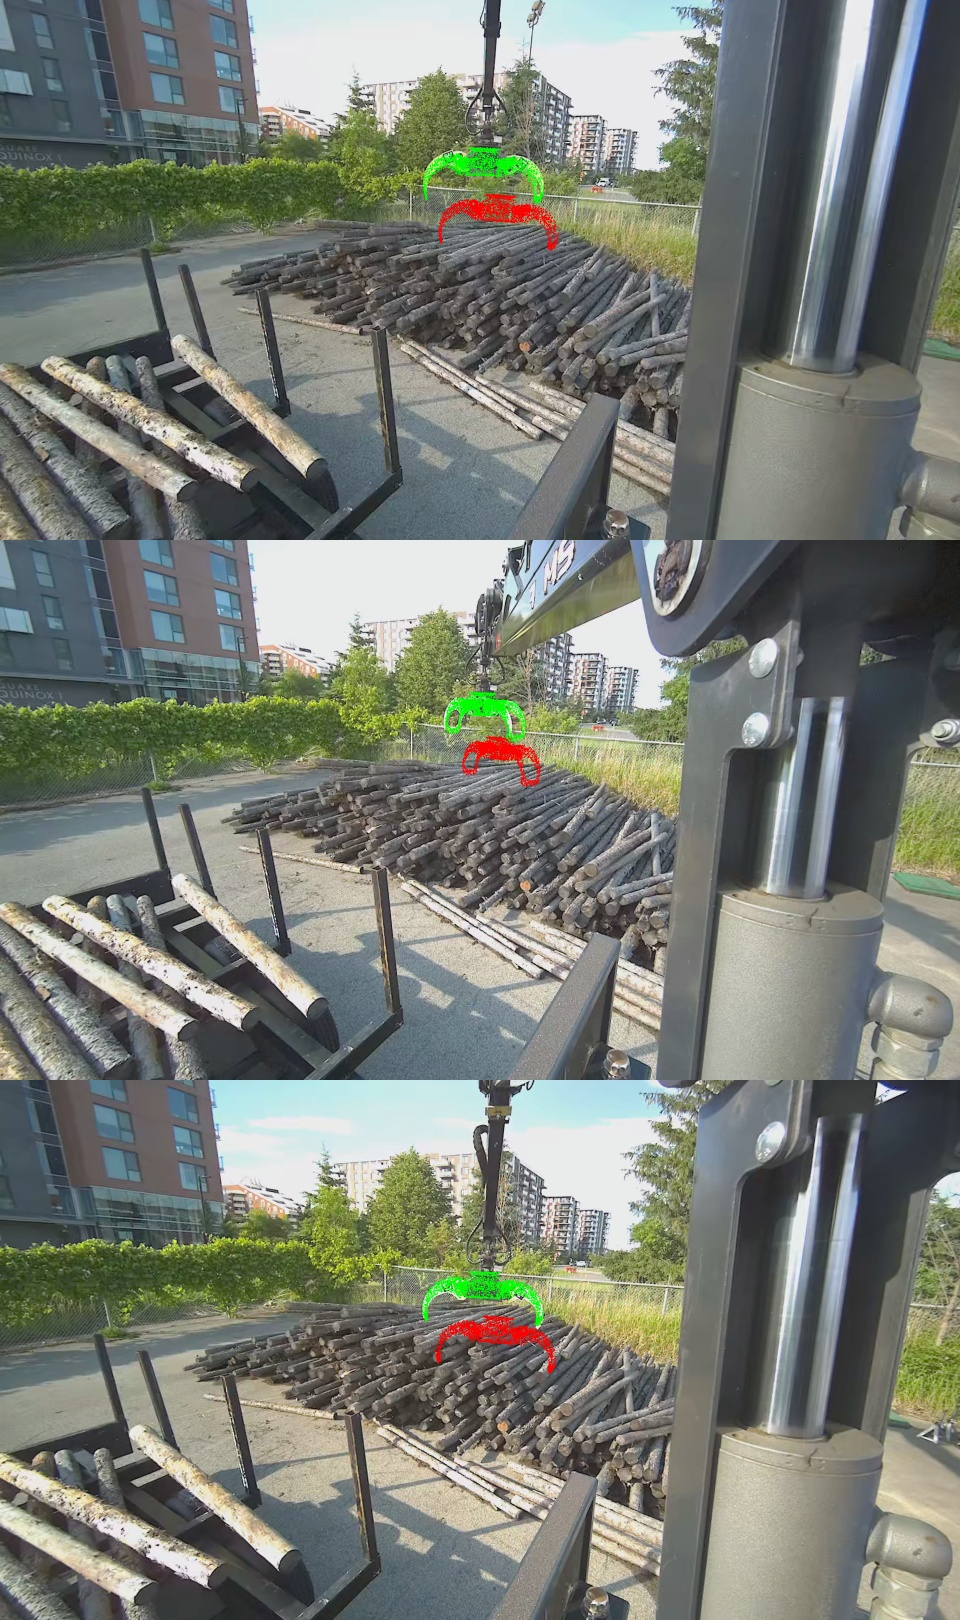
\includegraphics[height=0.72\textheight]{reproj_zed_0.jpg}\\
    {\tiny zed\_0: posed grapple CAD (\textcolor{successgreen}{green}) reprojected onto the observed grapple.}
  \end{column}
  \begin{column}{0.60\textwidth}
    \begin{block}{From William's render-and-compare}
      \footnotesize
      \begin{tightitemize}
        \item Rebuilt against \emph{our} URDF + STL meshes; FK validated to \textbf{0.0\,mm / 0.00$^\circ$} vs.\ bag \texttt{/tf}
        \item \textbf{zed\_1} calibrates in \texttt{stick}, \textbf{zed\_0} in \texttt{mast} (slew cancels in the cam$\to$grapple chain)
        \item Dense grapple clouds ($\sim$2300--3500 pts) from the motion bag ($\sim$1132 cropped clouds/cam available); the fit uses $\sim$24 evenly-sampled poses
      \end{tightitemize}
    \end{block}
  \end{column}
\end{columns}
\end{frame}

% ==================================================================
\begin{frame}{Rack Calibration: Fusing Both Cameras}
\vspace{-1mm}
\begin{columns}[c,totalwidth=\textwidth]
  \begin{column}{0.50\textwidth}
    \centering
    \resizebox{\textwidth}{!}{%
    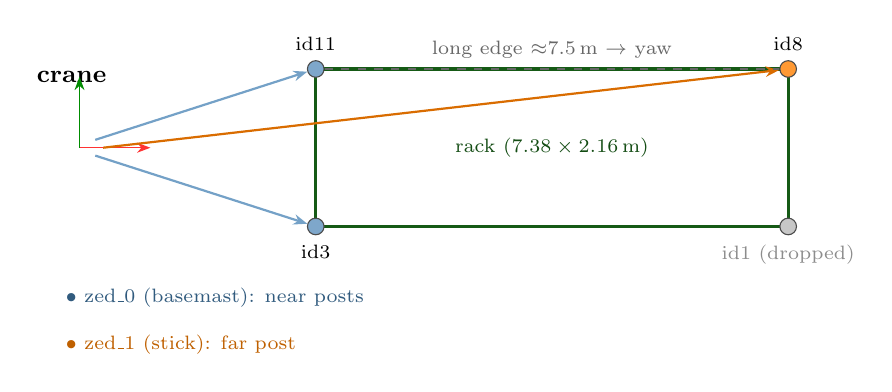
\begin{tikzpicture}[
      post/.style={circle, draw=black!70, minimum size=6pt, inner sep=0pt},
      z0/.style={post, fill=simblue!70},
      z1/.style={post, fill=orange!80},
      bad/.style={post, fill=black!22},
      lbl/.style={font=\scriptsize},
      arr0/.style={-{Stealth[length=5pt]}, simblue!75, thick},
      arr1/.style={-{Stealth[length=5pt]}, orange!85!black, thick},
    ]
      % crane base + frame
      \node[font=\small\bfseries] at (-0.1,1.9) {crane};
      \draw[-{Stealth}, red!80] (0,1) -- (0.9,1);
      \draw[-{Stealth}, green!55!black] (0,1) -- (0,1.9);
      % rack footprint
      \draw[successgreen!65!black, very thick] (3,0) rectangle (9,2);
      \node[lbl, successgreen!55!black] at (6,1) {rack ($7.38\times2.16$\,m)};
      % posts
      \node[z0,label={[lbl]below:id3}]  (id3)  at (3,0) {};
      \node[z0,label={[lbl]above:id11}] (id11) at (3,2) {};
      \node[bad,label={[lbl]below:{\color{black!45}id1 (dropped)}}] (id1) at (9,0) {};
      \node[z1,label={[lbl]above:id8}]  (id8)  at (9,2) {};
      % views
      \draw[arr0] (0.2,1.1) -- (id11);
      \draw[arr0] (0.2,0.9) -- (id3);
      \draw[arr1] (0.3,1.0) -- (id8);
      % cross-camera baseline
      \draw[dashed, thick, black!60] (id11) -- node[lbl,above,sloped]{long edge $\approx$7.5\,m $\to$ yaw} (id8);
      % legend
      \node[lbl, simblue!70!black, anchor=west] at (-0.3,-0.9) {$\bullet$ zed\_0 (basemast): near posts};
      \node[lbl, orange!75!black, anchor=west] at (-0.3,-1.5) {$\bullet$ zed\_1 (stick): far post};
    \end{tikzpicture}%
    }
  \end{column}
  \begin{column}{0.48\textwidth}
    \begin{block}{Coverage}
      \scriptsize
      The rack is 7.38\,m long; \textbf{no single camera} frames both ends with usable marker depth. Both cameras are calibrated into the \textbf{same base frame}, so markers seen by either one fuse into one rectangle.
    \end{block}
    \begin{block}{Marker $\to$ Base}
      \scriptsize
      \begin{tightitemize}
        \item Per marker: ArUco gives $T_{\text{cam}\leftarrow\text{marker}}$, lifted to base by $\text{FK}\cdot T_{\text{parent}\leftarrow\text{cam}}$ (the \textbf{calibrated} mount)
        \item zed\_0 $\to$ near posts \texttt{id3,id11}; zed\_1 $\to$ far post \texttt{id8}. \texttt{id1} dropped (stick extrapolates poorly to that very-near 2\,m marker, lands $\sim$1.3\,m high)
        \item Cross-camera long edge \texttt{id11}$\to$\texttt{id8} ($\approx$7.5\,m) $\to$ precise yaw $1.77^\circ$ (vs.\ $2.34^\circ$ from the short near edge)
        \item Post columns in the registered cloud fix corner XY (ArUco depth is the weak axis)
      \end{tightitemize}
    \end{block}
  \end{column}
\end{columns}
\end{frame}

% ==================================================================
\begin{frame}{Rack Calibration: Marker Detections}
\vspace{-1mm}
\begin{columns}[c,totalwidth=\textwidth]
  \begin{column}{0.47\textwidth}\centering
    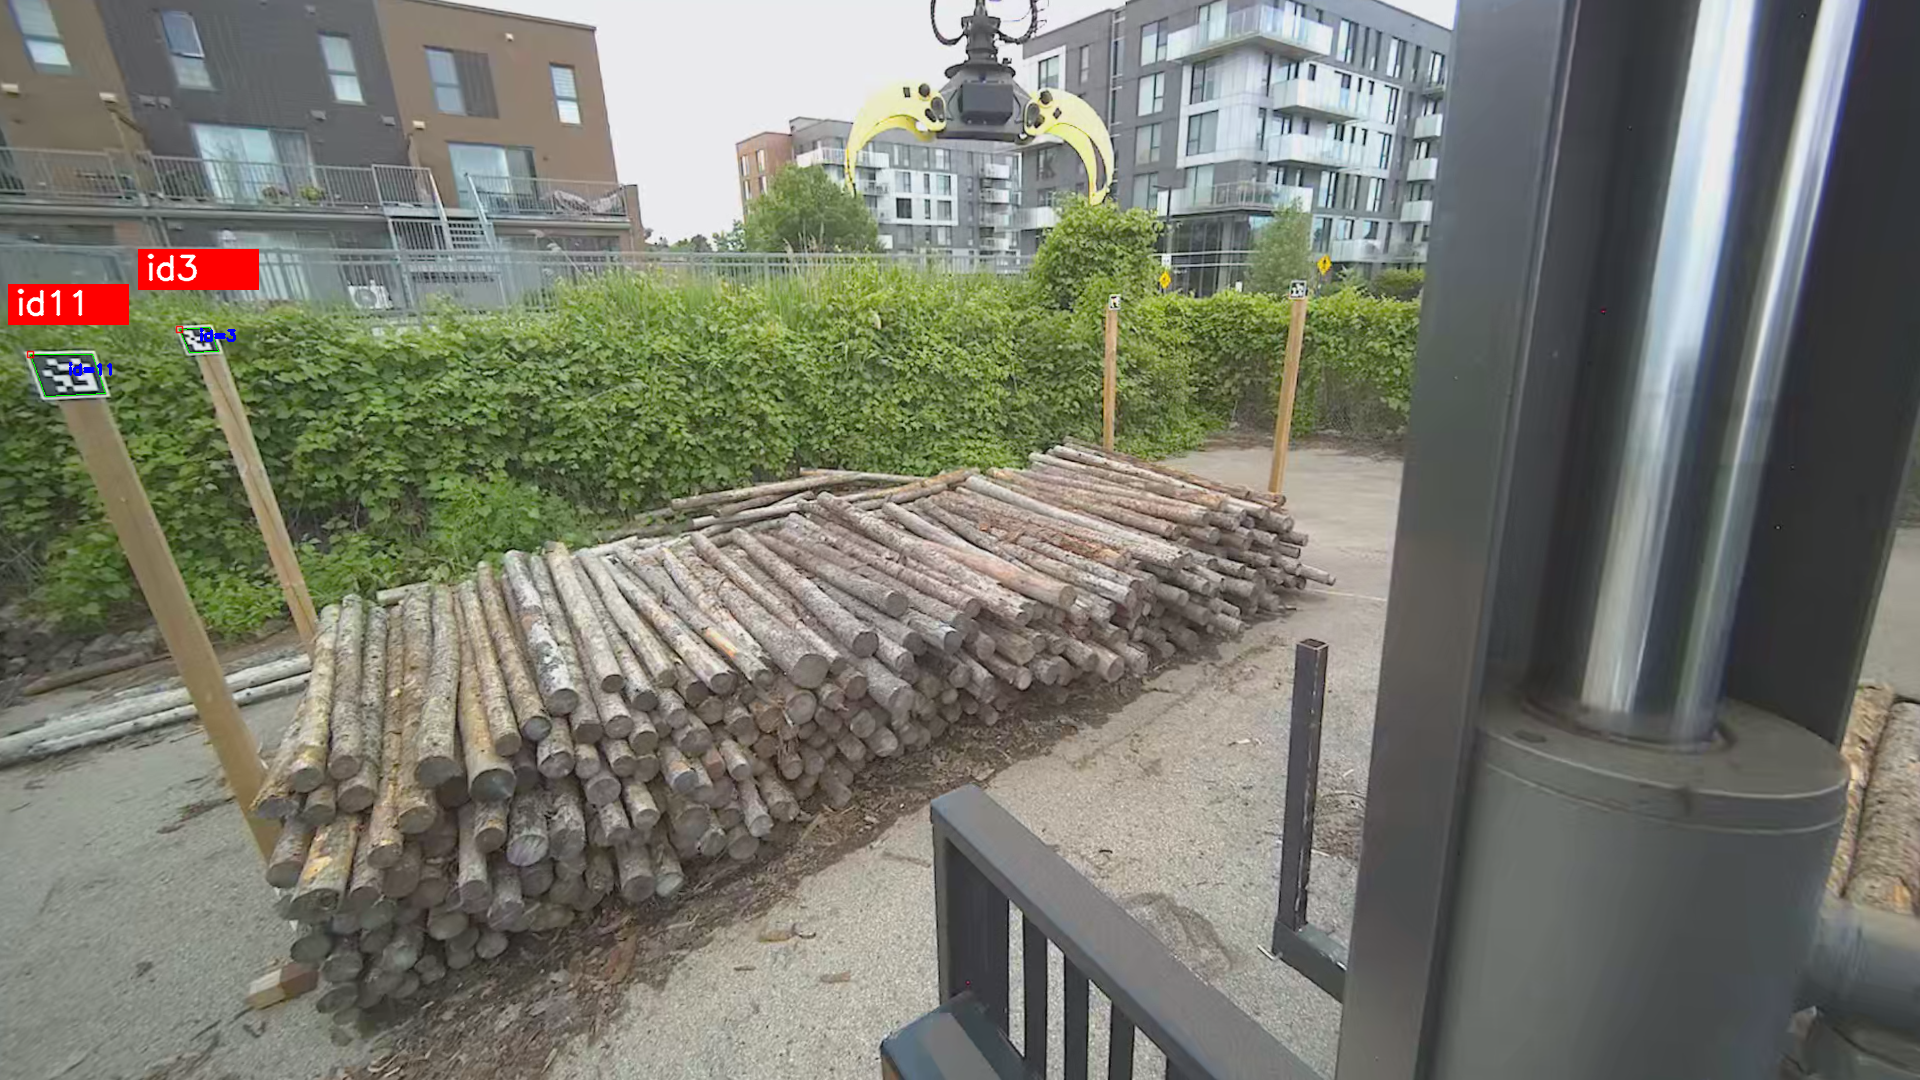
\includegraphics[width=\textwidth]{det_zed0.png}\\
    {\tiny Basemast (zed\_0): near posts \textbf{id3}, \textbf{id11}}
  \end{column}
  \begin{column}{0.47\textwidth}\centering
    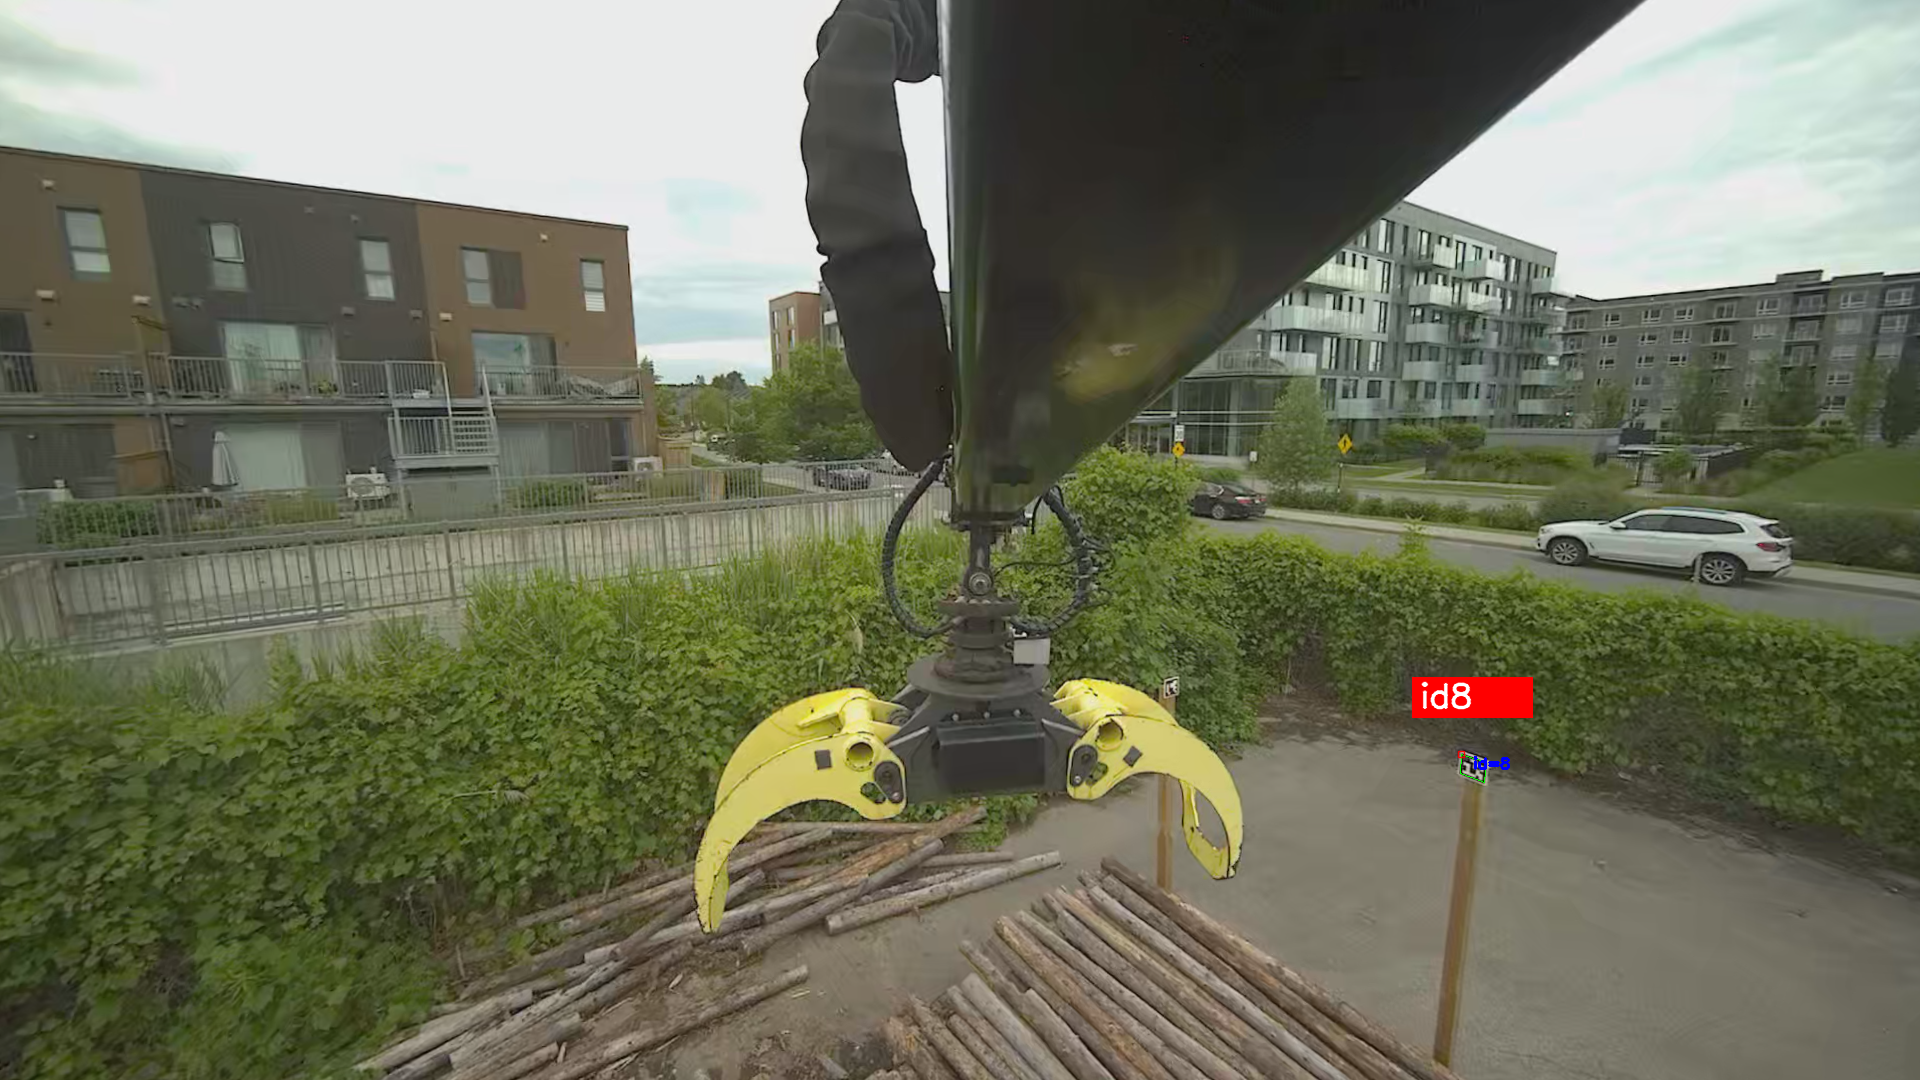
\includegraphics[width=\textwidth]{det_zed1.png}\\
    {\tiny Stick (zed\_1): far post \textbf{id8} (grapple in foreground)}
  \end{column}
\end{columns}
\vspace{1mm}
{\scriptsize ArUco (DICT\_6X6\_50) detected in each camera's full-resolution frame, then lifted to the base frame through that camera's calibrated extrinsic. Together the views span the rack's long edge (\texttt{id11}$\to$\texttt{id8}, $\approx$7.5\,m), giving a precise yaw.}
\end{frame}

% ==================================================================
\begin{frame}{Rack Calibration: Result}
\begin{columns}[c,totalwidth=\textwidth]
  \begin{column}{0.55\textwidth}
    \centering
    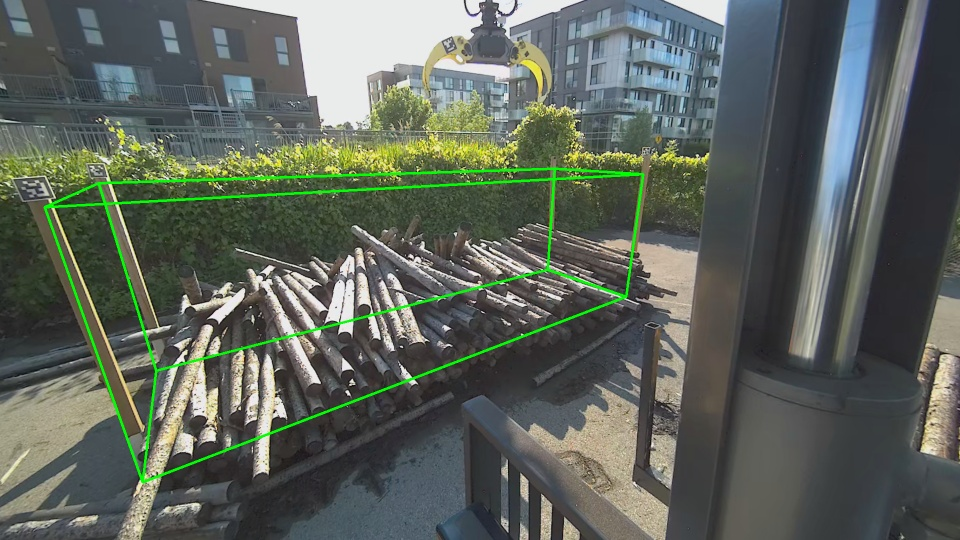
\includegraphics[width=\textwidth]{rack_final_wire7.jpg}\\
    {\tiny Calibrated rack box (\textcolor{successgreen}{green}) reprojected on the real basemast image; ArUco marker top-left.}
  \end{column}
  \begin{column}{0.43\textwidth}
    \begin{block}{Placed Rack}
      \footnotesize
      \begin{tightitemize}
        \item True dims $2.16\times7.38\times2.4$\,m
        \item Base pose: center $(-5.06,2.53,-1.42)$, yaw $1.77^\circ$
        \item Bottom set \textbf{flat on the floor} (markers showed only a $\sim$1--2$^\circ$ tilt, flattened for sim)
        \item Action bounds set \emph{inside} this box
      \end{tightitemize}
    \end{block}
    \begin{exampleblock}{Validation}
      \footnotesize
      The marker-derived rack bottom matches the sim ground plane to \textbf{24\,mm}, and the box edges follow the real posts in the image.
    \end{exampleblock}
  \end{column}
\end{columns}
\end{frame}

% ==================================================================
\begin{frame}{Updating the Sim to Match Real}
\begin{block}{Asset / Pose Updates}
  \footnotesize
  \begin{tightitemize}
    \item Three sensor mounts baked into the \textbf{URDF} (full chain reproduces to machine precision)
    \item Basemast ZED + LiDAR frame added to the \textbf{sim USD}, pinned kinematically to the mast
    \item Rack placed at the calibrated base pose; logs and \textbf{action bounds} set in the base frame
    \item Gaze slew set so the sim basemast cam frames the rack
  \end{tightitemize}
\end{block}
\end{frame}

% ==================================================================
\begin{frame}{Sim vs.\ Real: Gaze View}
\vspace{-1mm}
\begin{center}
  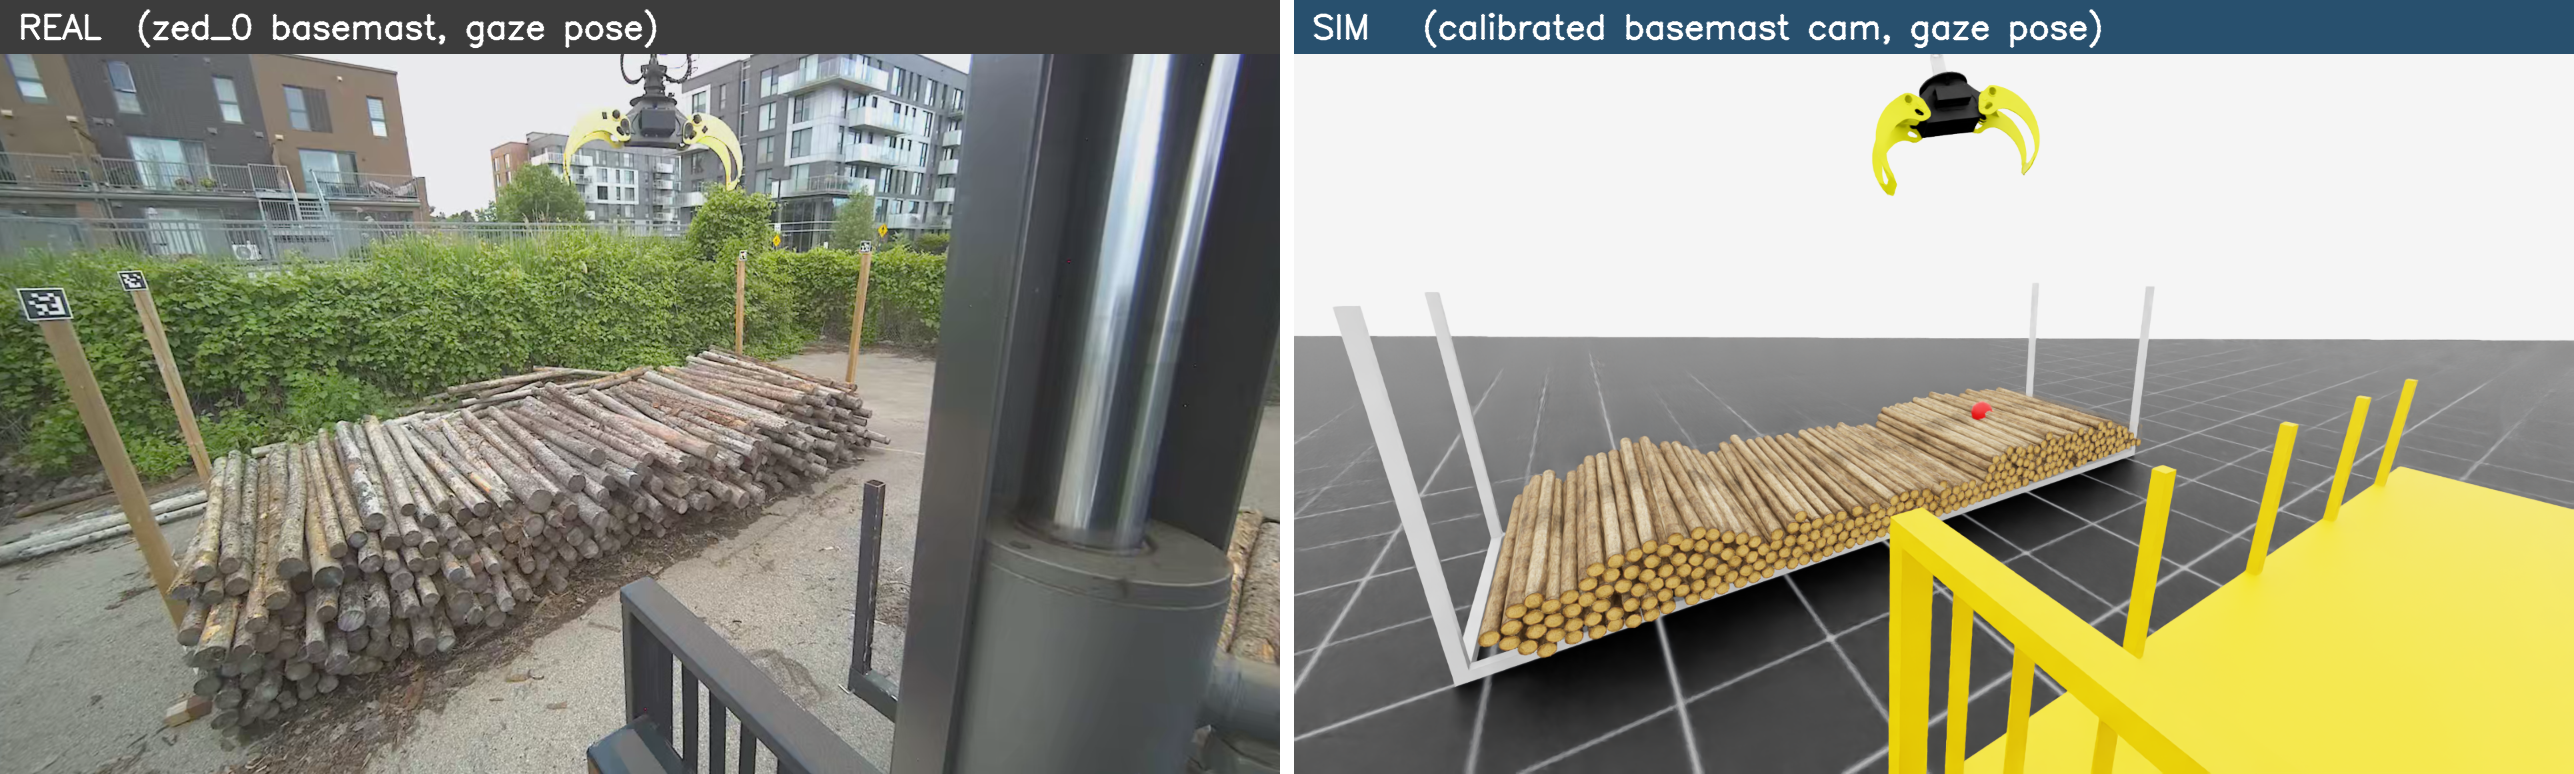
\includegraphics[width=0.96\textwidth]{gaze_real_vs_sim.png}
\end{center}
\vspace{-2mm}
{\scriptsize
Basemast (zed\_0) view at the gaze pose. The calibrated sim camera reproduces the real viewpoint: grapple top-center, log pile lower-left, rack frame, trailer right. This is the exact image the depth pipeline turns into the policy's point cloud.}
\end{frame}

% ==================================================================
\begin{frame}{Sim vs.\ Real: Point Cloud (Base Frame)}
\vspace{-1mm}
\begin{columns}[c,totalwidth=\textwidth]
  \begin{column}{0.34\textwidth}\centering
    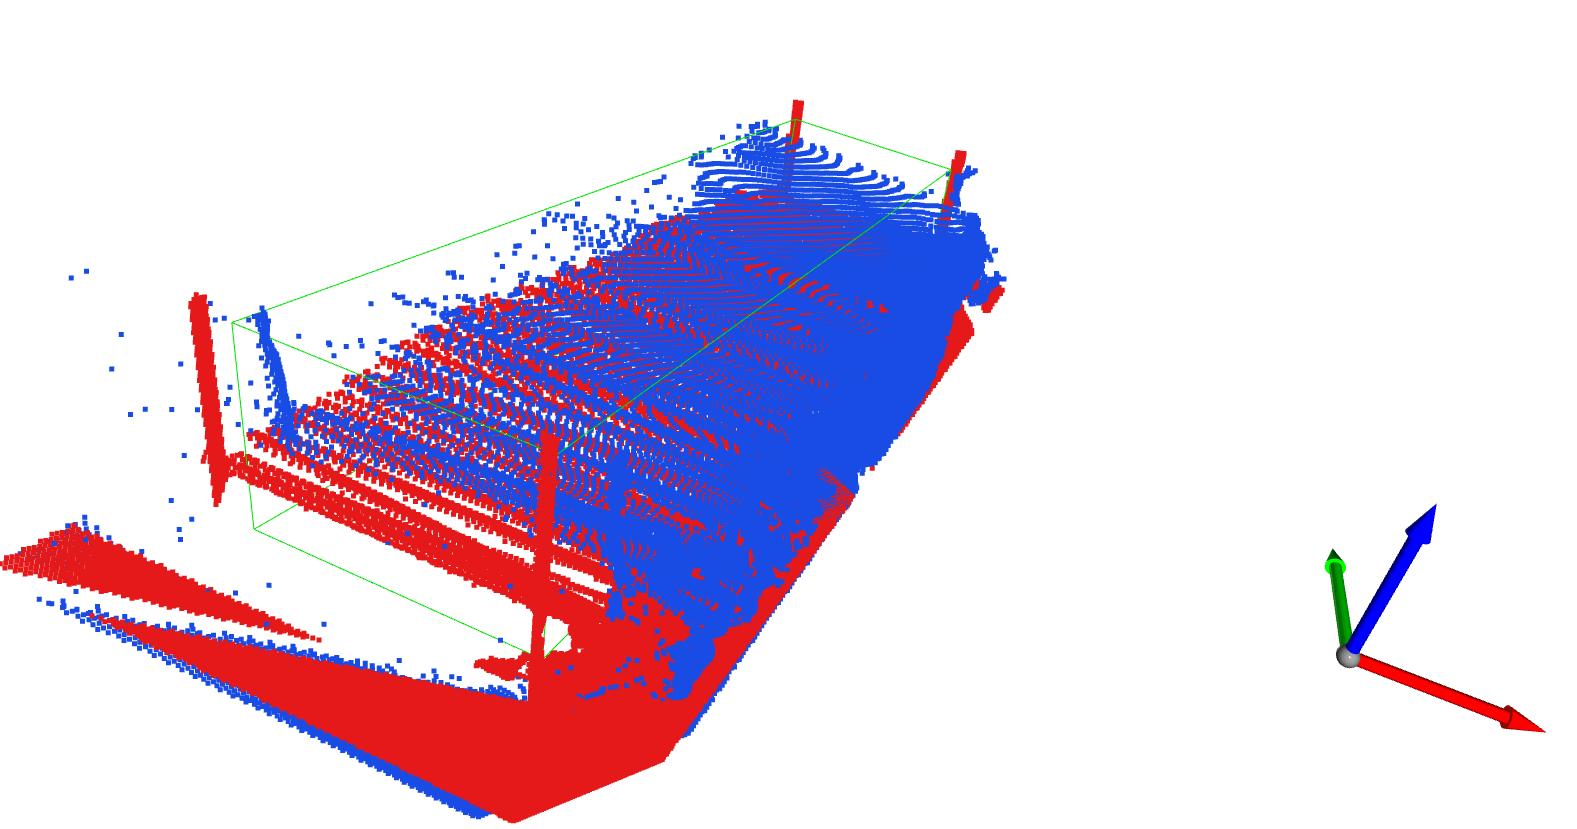
\includegraphics[width=\textwidth]{pcd_overlay_iso.png}\\{\tiny Isometric}
  \end{column}
  \begin{column}{0.30\textwidth}\centering
    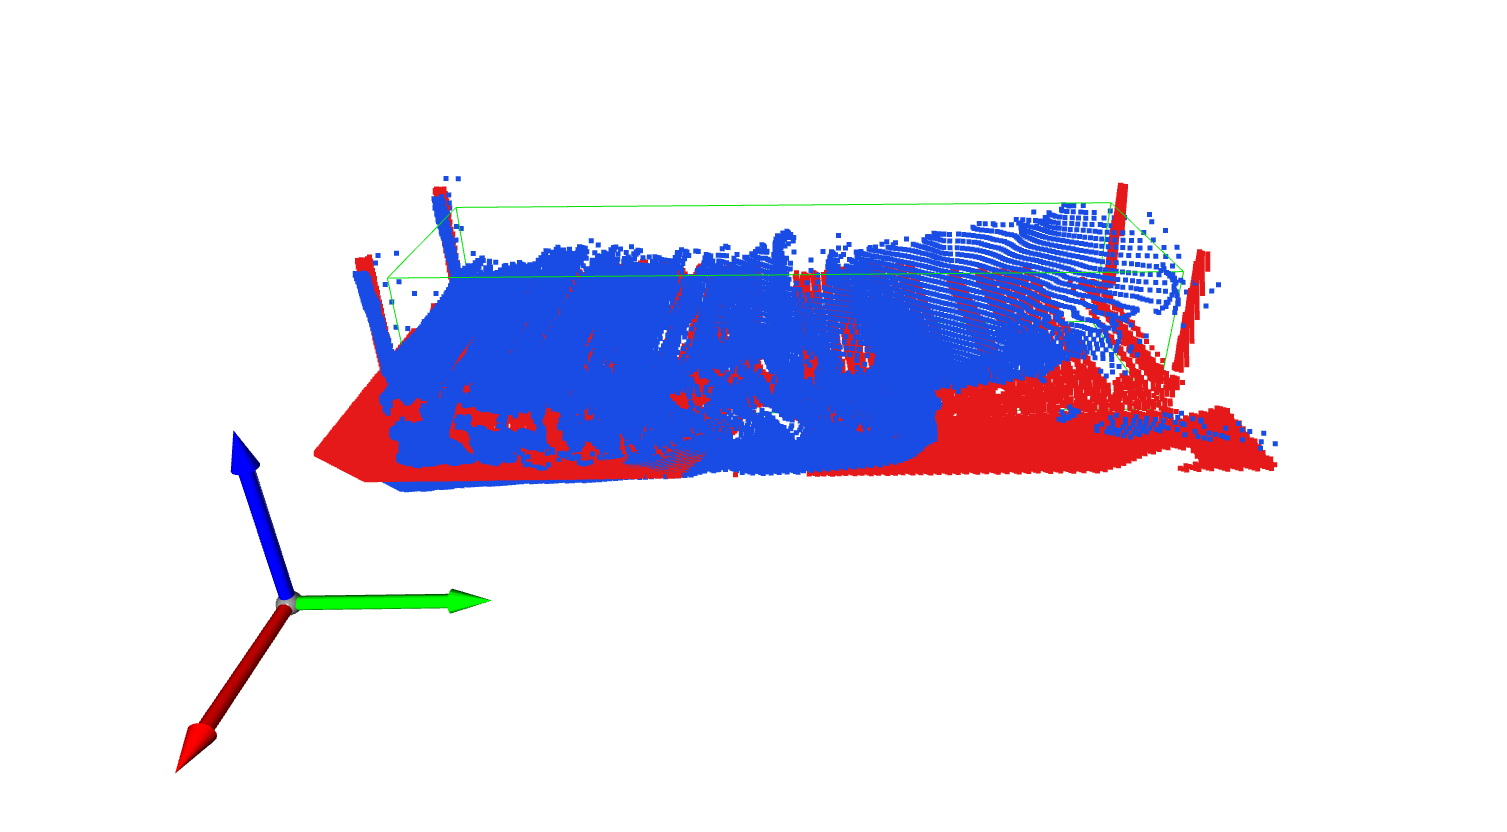
\includegraphics[width=\textwidth]{pcd_overlay.png}\\{\tiny Front profile}
  \end{column}
  \begin{column}{0.34\textwidth}\centering
    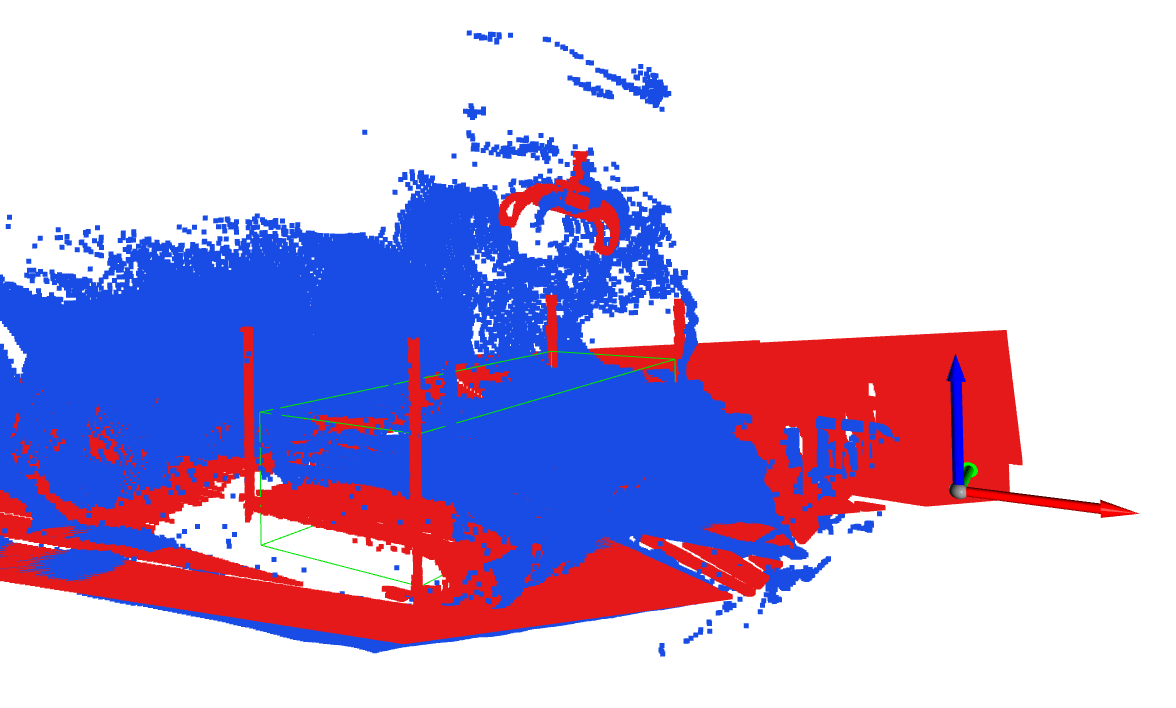
\includegraphics[width=\textwidth]{pcd_overlay_uncropped.png}\\{\tiny Full scene (uncropped)}
  \end{column}
\end{columns}
\vspace{1mm}
{\scriptsize
\textcolor{failred}{sim (red)} vs.\ \textcolor{simblue}{real (blue)}; \textcolor{successgreen}{action bounds (green)}. With the calibrated extrinsics the clouds land on the same rack in the base frame (shared extent $x\in[-6.9,-3.2]$, $y\in[-1.8,6.8]$). The uncropped view shows the grapple and background that the action-bounds crop removes before inference. Remaining gap: real stereo has holes / noise and the floor sits $\sim$13\,cm lower $\to$ depth-noise + point-dropout augmentation.}
\end{frame}

% ==================================================================
\begin{frame}{Next Steps}
\begin{block}{Plan}
  \footnotesize
  \begin{enumerate}\setlength{\itemsep}{3pt}
    \item Rebuild the sim pile to the ordered layout; finalize reachable action bounds
    \item \textbf{Train the BC policy in sim} on the calibrated gaze input
    \item Attempt \textbf{zero-shot transfer} to the real crane (rosbag replay $\to$ dry run $\to$ live)
    \item If transfer is poor: retrain with depth-noise / dropout / viewpoint augmentation
  \end{enumerate}
\end{block}
\end{frame}

% ==================================================================
\begin{frame}
  \centering
  \vspace{1.5cm}
  {\Huge\textbf{Questions?}}
  \vspace{8mm}

  {\large George Sideris}\\[3mm]
  {\small george.sideris@mail.mcgill.ca}\\[2mm]
  {\small McGill University, Aerospace Mechatronics Lab}\\[5mm]
\end{frame}

\end{document}
